% !TEX root = ../main.tex
%--- Slide 2: pulsar timing array (circa 1 min) ------------------------------------------
% Figure: Figure/P02_hellings_downs.pdf e Figure/P02_power_law.pdf (notebook 28).
\begin{frame}{Pulsar timing array}
  \small
  \begin{itemize}\setlength{\itemsep}{1pt}
    \item \textbf{Millisecond pulsar} (MSP): impulsi radio regolari come orologi atomici
    \item Un'onda gravitazionale tra la Terra e la pulsar fa arrivare gli impulsi
          in anticipo o in ritardo
    \item \textbf{Pulsar timing array}: si misurano per anni i tempi di arrivo (TOA) di molte pulsar,
          quindi si osservano onde a frequenze dei nHz
    \item Il fondo stocastico (\textbf{GWB}) è un segnale comune, \textbf{correlato tra le pulsar}
          (curva di Hellings--Downs). Prime evidenze nel 2023
    \item È un \textbf{processo stocastico} con spettro a \textbf{legge di potenza},
          $S(f) \propto A^2 (f/\fyr)^{-\gamma}$, come i rumori della pulsar
  \end{itemize}
  \vspace{1mm}
  \centering
  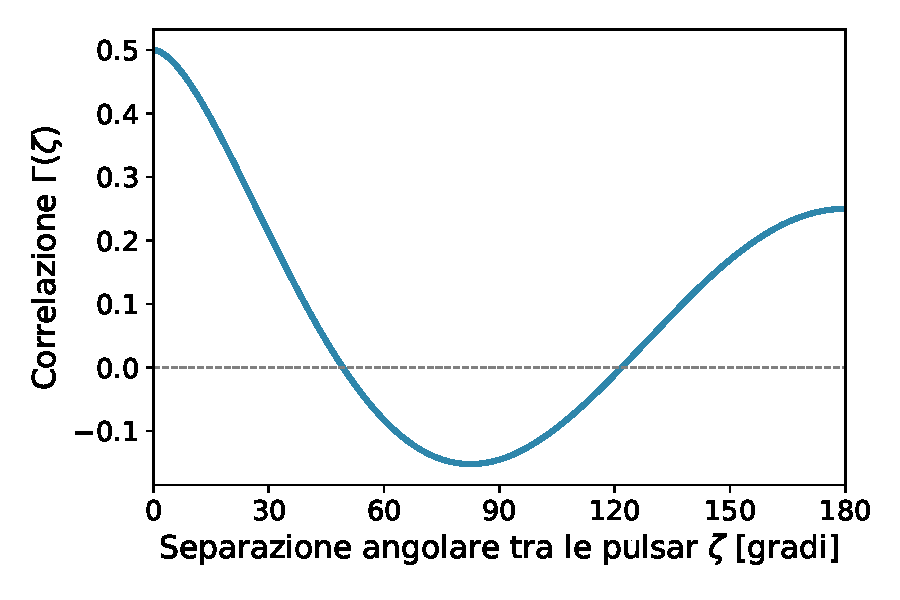
\includegraphics[height=0.38\textheight]{Figure/P02_hellings_downs.pdf}\hfill
  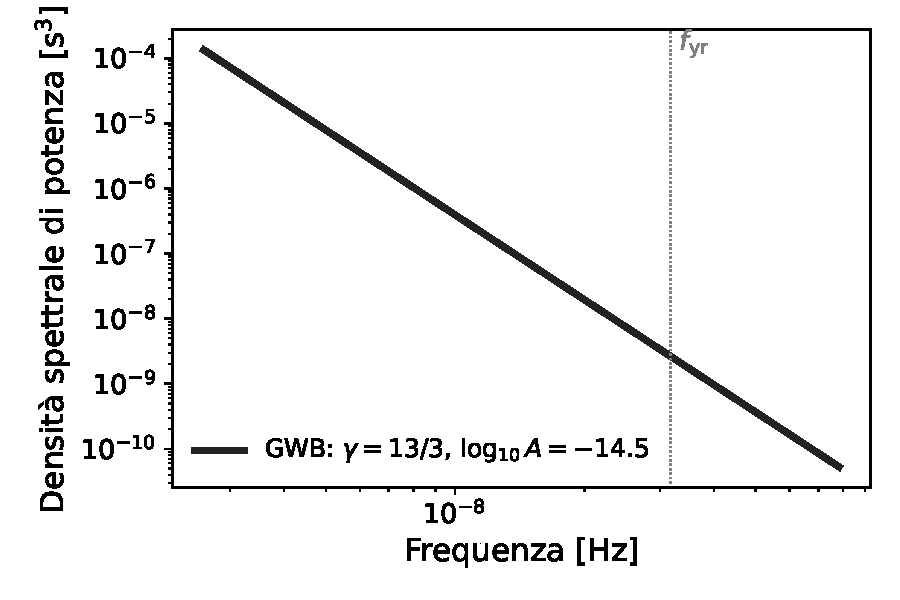
\includegraphics[height=0.38\textheight]{Figure/P02_power_law.pdf}
\end{frame}
